\documentclass[18pt]{article}
\usepackage[utf8]{inputenc}
\usepackage[T1]{fontenc}
\usepackage{ragged2e}
\usepackage{caladea}
\usepackage{graphicx}
\usepackage{longtable}
\usepackage{wrapfig}
\usepackage{rotating}
\usepackage{epigraph}
\usepackage[normalem]{ulem}
\usepackage{hyperref}
\usepackage{amsmath}
\usepackage{amssymb}
\usepackage{capt-of}
\usepackage{hyperref}
\usepackage{fancyhdr}

\title{
 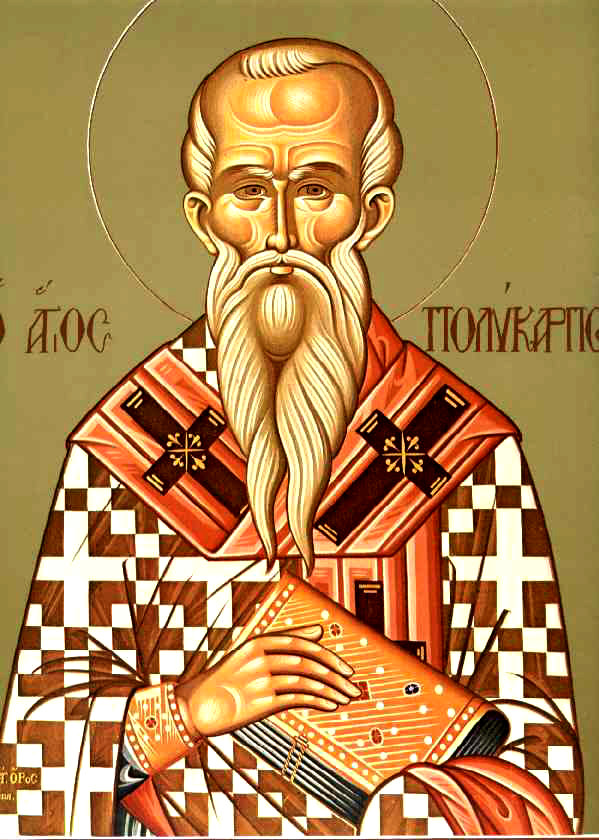
\includegraphics[scale=3.6, trim={10cm, 0, 10cm, 0}]{./assets/imagem.jpg}
  \par
   NOVENA A SÃO POLICARPO DE ESMIRNA}
\date{Início da Novena: 14/02 - Data Litúrgica: 22/02 }

% Comando para fazer "Sumário" não aparecer no Sumário.
\renewcommand{\contentsname}{Sumário}
\begin{document}
\maketitle

\thispagestyle{empty} %zera a primeira página

\pagestyle{fancy}
\fancyhf{} % clear existing header/footer entries
\fancyfoot[LO, CE]{

\includegraphics[scale=0.2]{./assets/cross.png} São Policarpo de Esmirna, rogai por nós!
}
% Place Page X of Y on the right-hand
% side of the footer
\fancyfoot[R]{\thepage}

\newpage

\tableofcontents

\centering
\vfill
Visite-nos no Telegram: \url{https://t.me/CotidieNovena}
\newpage

\newpage


%%%%%%%%%%%%%%%%%%%%%%%%%%%%%%%%%%%%% Orações %%%%%%%%%%%%%%%%%%%%%%%%%%%%%%%%%%%%%%%%%%%

\begin{justify}

 \begin{center}
  \section{História}\label{sec:História} % (fold)
 \end{center}


 \begin{justify}
  \subsection{Origens Grande padre apóstolo}
 \end{justify}

São Policarpo está entre os grandes padres apostólicos, ou seja, pertencia ao número daqueles que conviveram com os primeiros apóstolos e serviram de elo entre a Igreja primitiva e a Igreja do mundo greco-romano.

São Policarpo foi ordenado Bispo de Esmirna pelo próprio São João, o Evangelista. De caráter reto, de elevado saber, amor à Igreja e fiel à ortodoxia da fé, era respeitado por todos no Oriente.

A carta escrita por Policarpo aos Filipenses foi preservada. Nesta carta, ele diz: “Fique firme, e na sua conduta siga o exemplo do Senhor, firme e imutável em sua fé, ame seu irmão, amando a cada um e a todos, unidos na verdade e ajudando a cada um com a bondade do Senhor Jesus, não desprezando a nenhum homem”.

\begin{justify}
 \subsection{São Policarpo e a perseguição aos cristãos}
\end{justify}

Reação de impacto
Com a perseguição aos cristãos, o santo bispo de 86 anos escondeu-se até ser preso e levado para o governador, que pretendia convencê-lo de ofender a Cristo. Policarpo, porém, proferiu estas palavras: “Há oitenta e seis anos sirvo a Cristo, e nenhum mal tenho recebido dele. Como poderei rejeitar Aquele a quem prestei culto e reconheço como meu Salvador?”.


\vspace{.8cm}
\begin{justify}
 \subsection{Páscoa}
\end{justify}

Condenado à morte no estádio da cidade de Esmirna, na província da Ásia, na atual Turquia, ele próprio subiu na fogueira e testemunhou para o povo: “Sede bendito para sempre, ó Senhor. Que o Vosso Nome adorável seja glorificado por todos os séculos”. Milagrosamente, as chamas não o machucavam, e ele continuava a cantar. Impressionados, os guardas chamaram um arqueiro para que ele perfurasse o santo com uma flecha. Ao ser atingido, seu sangue apagou as chamas. Os guardas tentaram de novo acender a pira, mas sem sucesso. O encarregado do martírio, furioso, ordenou que Policarpo fosse decapitado.

\begin{justify}
 \subsection{São Policarpo: muitos frutos}
\end{justify}

Curiosidade sobre o nome
São Policarpo viveu o seu nome: poli = muitos; carpo = fruto | muitos frutos, que foram regados com suor, lágrimas e, no seu martírio, no ano de 155, regado também com sangue.

\begin{justify}
 \subsection{Segundo a tradição}
\end{justify}

Por tratar-se de um santo do segundo século, as informações sobre ele nem sempre são precisas, e neste caso, segue-se a tradição. Acredita-se que Policarpo foi um dos primeiros organizadores do que hoje para nós é o Novo Testamento.


\vfill

\begin{center}
 \href{https://www.praymorenovenas.com/st-margaret-of-cortona-novena}{Fonte: Pray More Novenas}
\end{center}

%%%%%%%%%%%%%%%%%%%%%%%%%%%%%%%%%%%%% Orações %%%%%%%%%%%%%%%%%%%%%%%%%%%%%%%%%%%%%%%%%%%

\newpage
\begin{center}
 \section{Orações}\label{sec:Orações} % (fold)
\textit{Em nome do Pai, e do Filho, e do Espírito Santo. Amém.}
\end{center}

\subsection{Oração Incial}\label{sec:Oração_Inicial} % (fold)



Deus de toda a Criação, você deu a seu Bispo, Policarpo, o privilégio de ser contado entre os santos que deram suas vidas em testemunho fiel ao evangelho. Que as suas preces nos deem a coragem de compartilhar com ele o cálice do sofrimento e ascender à glória eterna. Pedimos isso por nosso Senhor Jesus Cristo, seu Filho, que vive e reina contigo e com o Espírito Santo, um só Deus, para sempre e sempre.

\subsection{Oração Final}\label{sec:Oração_Final} % (fold)
\begin{center}
\textbf{Pai Nosso, Ave Maria, Glória ao Pai.}

\vfill
\section*{São Policarpo, Rogai por Nòs!}

\vfill
\subsection*{Créditos:}
\href{https://catholicnovenaapp.com/novenas/st-margaret-of-cortona-novena/#day-1-prayer}{Catholic Novena App}

\end{center}


\end{justify}

\end{document}
